%!TEX ROOT = thesis.tex
\chapter{Design}
\section{Introduction}
In this project, the driving behaviour analysis method contains driving operation data acquisition module, data preprocessing module, data fusion module and K Means algorithm module. The raw data will be preprocessed. Each driver's vehicle telemetry data will be concatenated into a single CSV file. The new CSV file will be categorized to three group by using K Means algorithm. Figure \ref{fig:projectflow} shows the flow of entire project.

\begin{figure}[hbt!]\centering
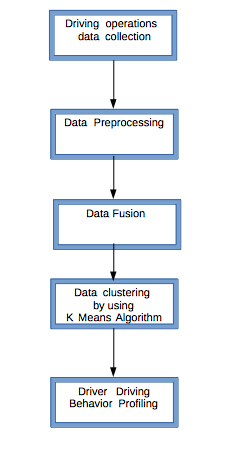
\includegraphics[height=.4\textheight]{image/flowchart}
\caption{The flow of the driver driving behaviour profiling method. }
\label{fig:projectflow}
\end{figure}

\section{Data Acquisition}
In this project, few drivers have been invited to participate in the data collection. The ELM327 device needs to be connected with the vehicle OBD-II socket. The smartphone with the Torque(Lite) needs to be put in the vehicle. It needs to connect with the ELM327 device and GPS location service. Torque(Lite) logging function needs to be triggered and stopped in each driver driving session. 

Vehicle telemetry data will be recorded in every second. The drivers are requested to drive at least 8 minutes. At least 480 vehicle operation records can be collected from each driver. All drivers were driving in different path. The raw data will be uploaded and stored in Google Drive. Figure \ref{fig:GDfile} shows  the view of the raw data in Google Drive.

\begin{figure}[hbt!]\centering
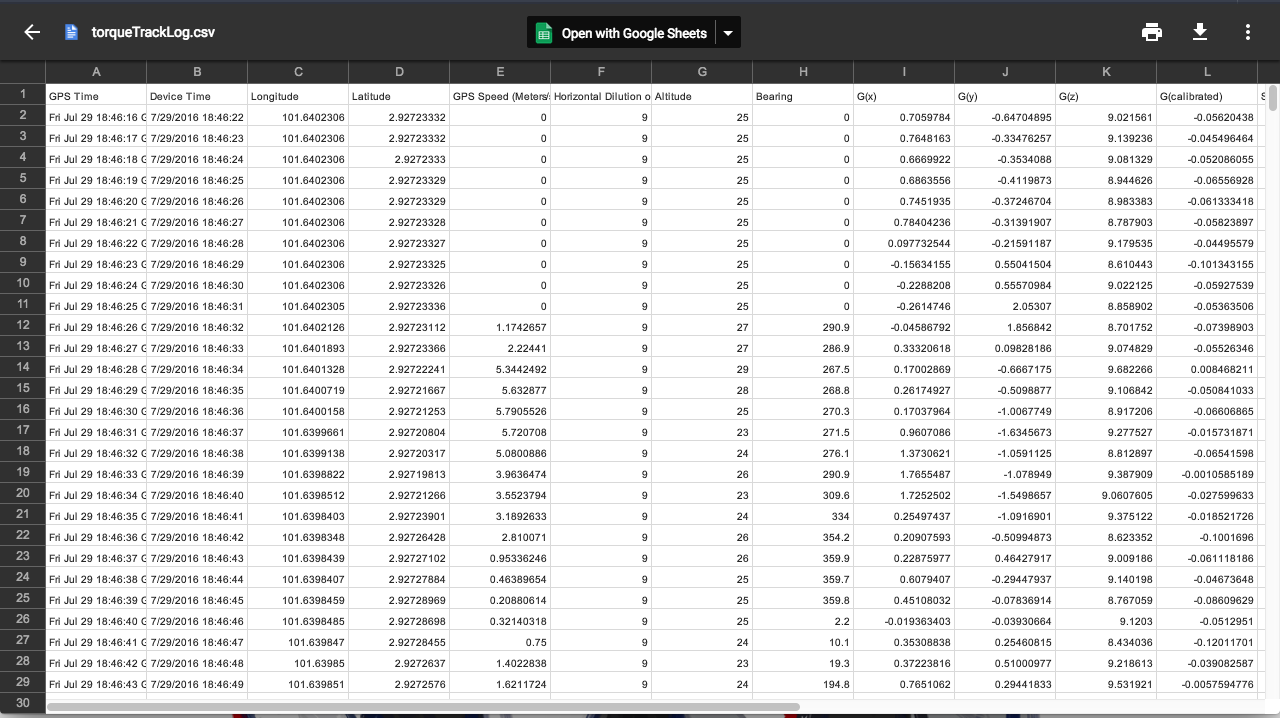
\includegraphics[width=.75\textwidth]{image/GDfile}
\caption{The raw data file is opened in Google Drive.}
\label{fig:GDfile}
\end{figure}

For this project, the vehicle OBD-II information data and GPS data will be collected and store in the same file. Some of the features are vehicle speed, engine speed, engine coolant temperature, throttle position, latitude coordinate, longitude coordinate, GPS speed, GPS altitude, horizontal dilution of precision, GPS bearing, and GPS acceleration. Those data will be written in a same file.

A new feature, speed test can be added into the data. Speed test is a value to determine whether the driver exceeded the speed limit or not at the particular time frame. The value of the speed test is '-1' or '1'. '-1' means the driver exceeded the speed limit at the particular time frame. '1' is on the contrast. The speed limit will be determined by the road condition. The road condition includes straight road, curve road, traffic light intersection, intersection, roundabout, and state road. The road condition will be referred from the Google Earth. The KML file converted by the Torque(Lite) will show the path of the driver drove. In Figure \ref{fig:GEMap}, each record of the vehicle telemetry data will be displayed as a green arrow and marked on the map. 

\begin{figure}[hbt!]\centering
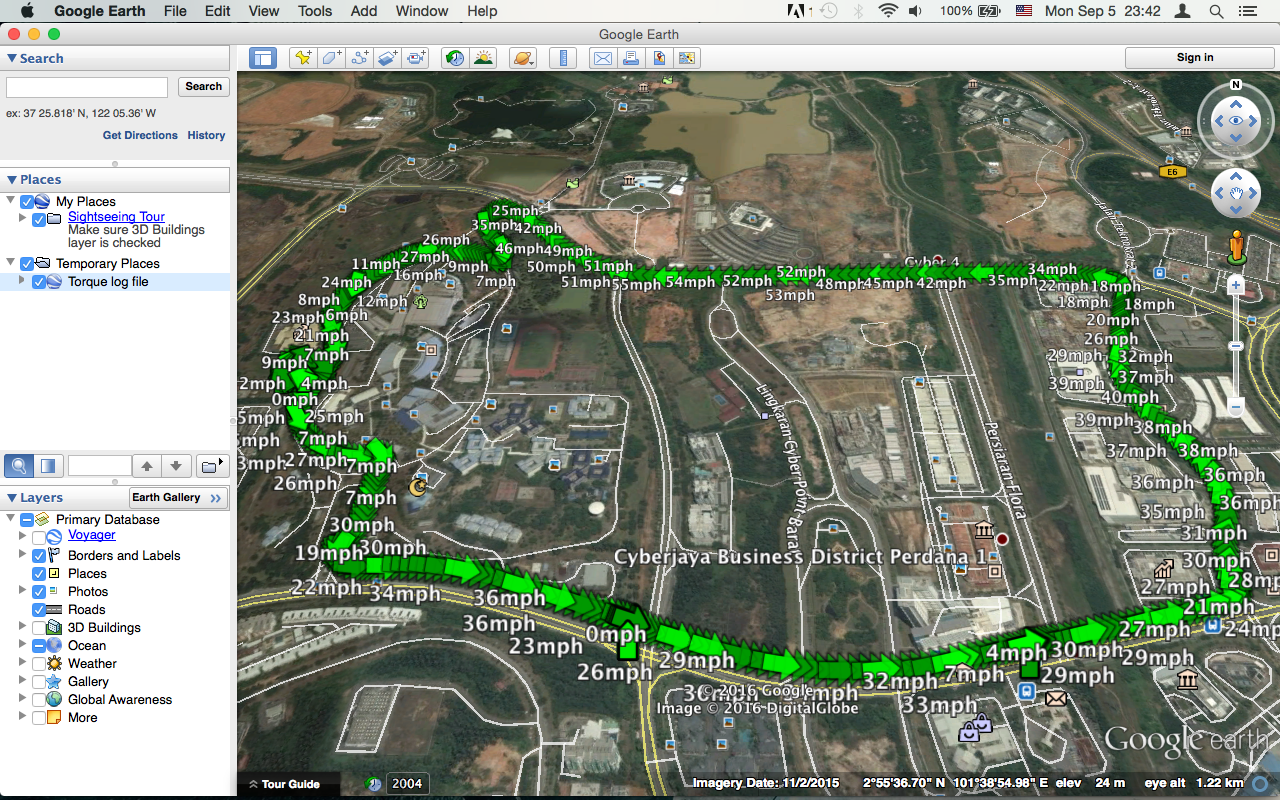
\includegraphics[width=.75\textwidth]{image/GEMapView}
\label{fig:GEMap}
\caption{The Map View in Google Earth for the vehicle telemetry data.}
\end{figure}

In order to identify the intersection on straight road or differentiate the traffic light intersection and normal intersection, Google Earth provided the Street View function that allows to observe the surroundings of the particular place. In Figure \ref{fig:GEStreet}, one of the traffic light intersection examples displayed in Google Earth. 

\begin{figure}[hbt!]\centering
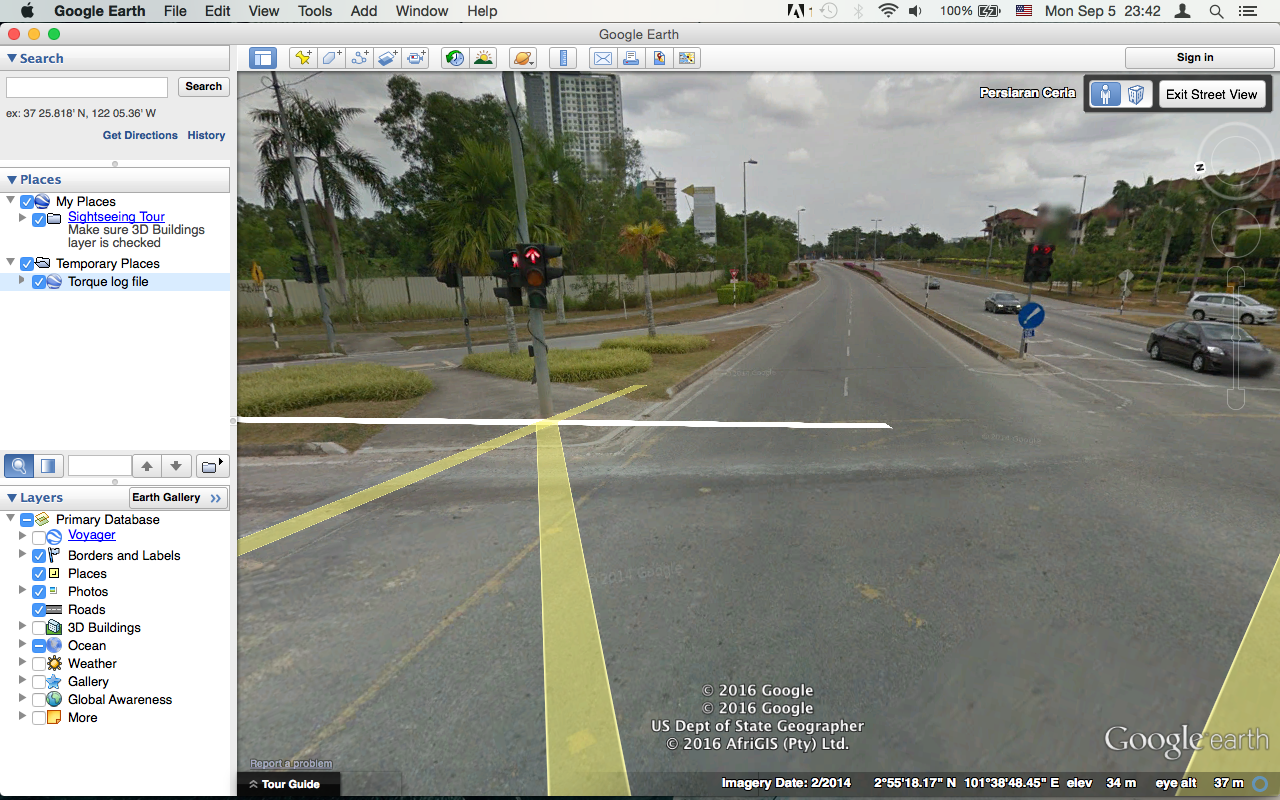
\includegraphics[width=.75\textwidth]{image/GEStreetView}
\caption{The Street View in Google Earth at the traffic light intersection.}
\label{fig:GEStreet}
\end{figure}

In Malaysia, speed limit of express ways by default is 110 km/h, but it will be 90km/h in crosswind area, mountainous stretches area, and urban area. Speed limit of state road or federal road is 80km/h, town area will be 60km/h. Due to some road condition, a 40km/h or 50km/h speed limit sign board will be placed in the area of having curve road. 

Drivers suppose to stop at the intersection and observe the surroundings vehicle movement before turning to the another route. So, speed limit of intersetcion area will be set as 30km/h in this project to determine the drivers' speed limit condition. The intersections having traffic light will be applied with 35km/h speed limit. Drivers should not drive through the traffic light intersection area with high speed. In some circumstances, the driver will accelerate when the traffic light changes to amber. As the result, the driver will stop the car uncomfortably due to this insufficient time period. The driver need to make decision at the stop-line either to pass through the intersection after red signals or brake hard in front of the intersection. This action will increase the potential of accident occurances.\cite{kulanthayan:phang:hayati:2007}

LibreOffice and Google Sheet are used to add on the speed test feature and the road condition feature. The driver name is also added to the vehicle telemetry data of the particular driver. Figure \ref{fig:speedtest} shown the vehicle telemetry data after added on new features.

\begin{figure}[hbt!]\centering
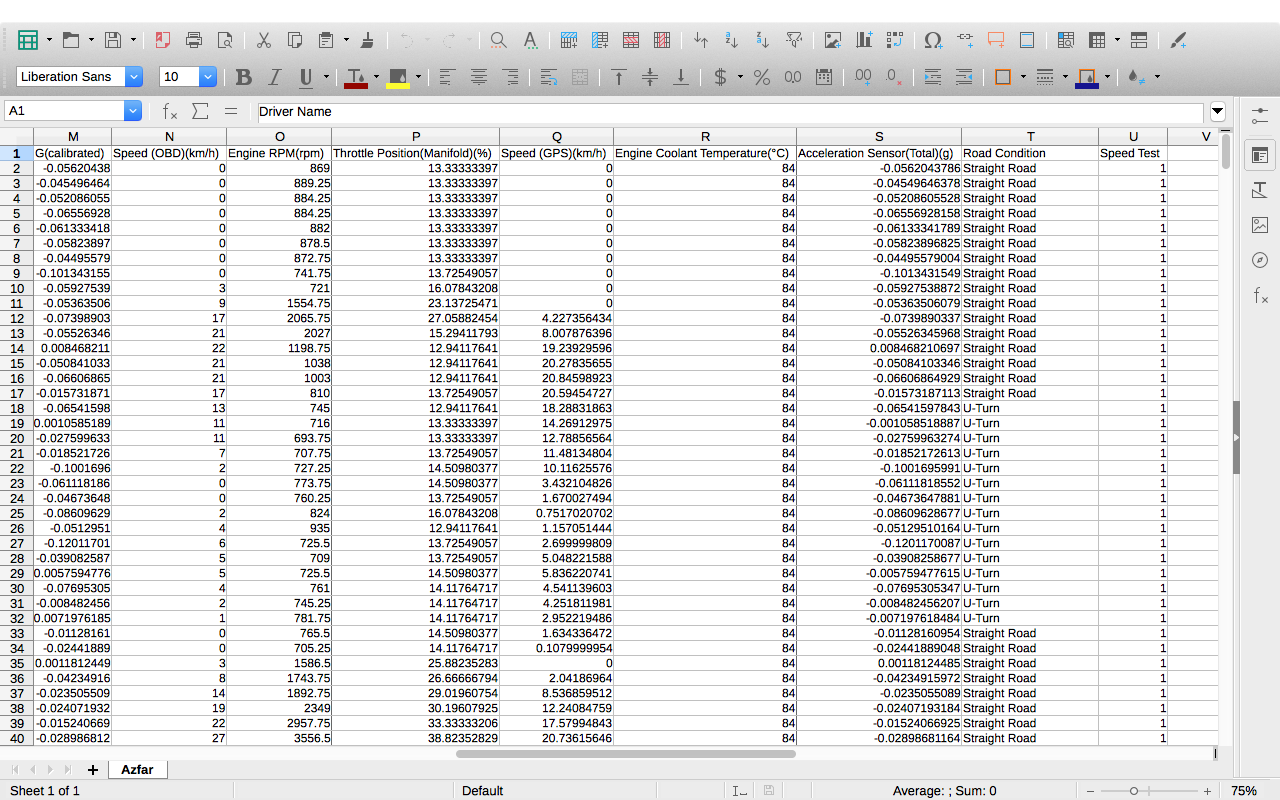
\includegraphics[width=.75\textwidth]{image/LOspeedtest}
\caption{The vehicle telemetry data is added on the speed test column and road condition column.}
\label{fig:speedtest}
\end{figure}


\section{Driving Operation Data Preprocessing}
The first 30 rows and last 30 rows of the collected vehicle telemetry data need to be removed. This is because drivers just come out from the parking at the beginning or drive into a parking slot at the end of the driving session. The removed data is always incomplete. Figure \ref{fig:preprocess} shows the setting of CSV Reader module of the KNIME Analytic Platform to perform data preprocessing.

\begin{figure}[hbt!]\centering
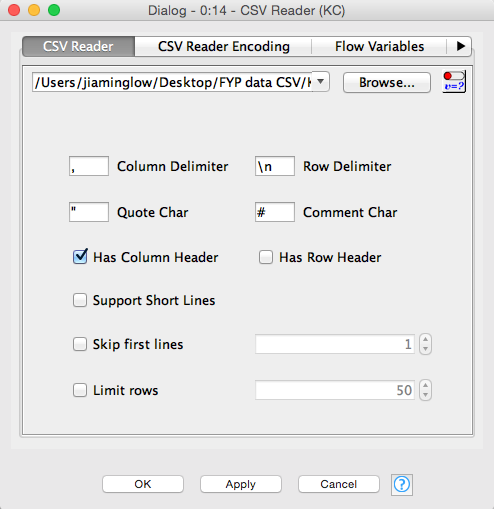
\includegraphics[width=.75\textwidth]{image/datapreprocessing}
\caption{CSV Reader settings for data preprocessing.}
\label{fig:preprocess}
\end{figure}

\section{Data Fusion}
All the pieces of preprocessed data for each driver are required to be concatenated as a big table before performing clustering. In Figure \ref{fig:KNIMEfile}, the processed data are concatenated by the concatenation module provided by KNIME.

\begin{figure}[hbt!]\centering
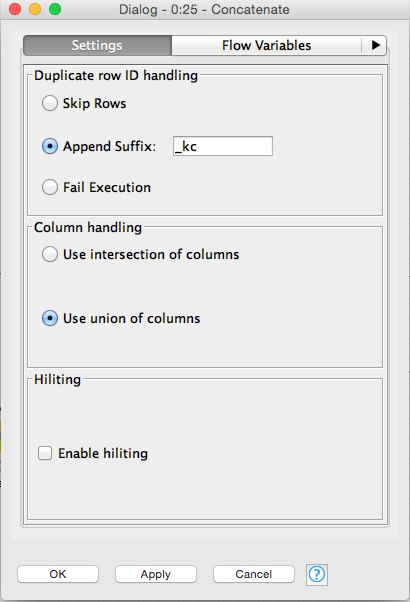
\includegraphics[width=.75\textwidth]{image/KNIMEconcatenate}
\caption{CSV files are concatenated by using the concatenation module in KNIME.}
\label{fig:KNIMEfile}
\end{figure}

\section{Establish the driving operation model by K Means Algorithm}
A work flow is designed and implemented by using KNIME Analytic Platform. The work flow will be able to input the vehicle telemetry data file and perform K Means Algorithm on the dataset. The number of clusters can be 3, 4, 5 or more. However, three clusters will be identified through the work flow in this project. The three clusters will represent the good, medium, and bad vehicle condition data. In the end of this process, each vehicle operation record will be labelled with the good, medium, and bad vehicle condition data.

\subsection{Features selection}
Some of the features of the vehicle telemetry data is chosen to be used in clustering. Linear Correlation module is implemented to help features selection. The linear correlation between the features are shown in Figure \ref{fig:correlation}. The low saturation of the colors means that the correlation between the two features is low. According to the correlation result, the selected features include GPS Altitude, GPS Bearing, GPS Vehicle Speed (km/h), Engine Speed, Throttle Position, and Speed Test. Engine coolant temperature and acceleration sensor is removed as these two features do not have strong relationship among the rest of the features. The selected features will be used in clustering.

\begin{figure}[hbt!]\centering
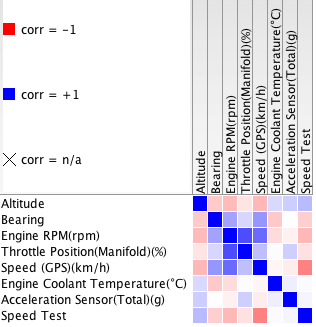
\includegraphics[height=.5\textwidth]{image/KNIMEcorrelation}
\caption{The correlation among the features}
\label{fig:correlation}
\end{figure}

\subsubsection{Linear Correlation}
Linear correlation is the straight line relationship between two variables. The range of the value of the linear correlation is between '-1' and '1'. If the value is '1', it means that the relationship is perfect positive relationship. The coordinates of the variables displayed on graph will be similar to a straight line with positive gradient. If the value is '-1', it means that the relationship is perfect negative relationship. The coordinates of the variable displayed on graph will be similar to a straight line with negative gradient. The '0' means no straight line relationship between the two variables.

\subsection{Cluster Labelling}
After the K Means Algorithm module execution, three clusters will be generated. Figure \ref{fig:cluster} shows the center coordinate of each cluster. An assumption is made at this point for giving the value to the clusters. According to the coordinates, speed test value is considered to label the clusters. 'cluster\_0' is assumed as good vehicle condition data as the speed test value of the coordinate is near to '1'. Most of the driving sessions are observed. Most of the drivers drove the car as normal and did not have dangerous actions performed. So, 'cluster\_2' is assumed as medium vehicle condition data due to the larger amount of the records under this cluster. 'cluster\_1' is assumed as bad vehicle condition data.

\begin{figure}[hbt!]\centering
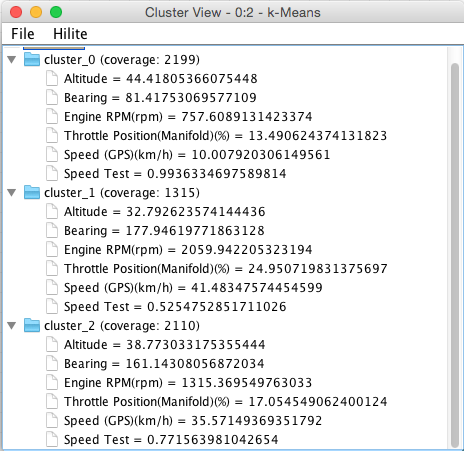
\includegraphics[height=.5\textwidth]{image/cluster}
\caption{The coordinates of cluster center for each cluster.}
\label{fig:cluster}
\end{figure}


String Replacer module provided by KNIME Analytic Platform is implemented to change the 'cluster\_0', 'cluster\_1' and 'cluster\_2' to 'good', 'medium' and 'bad' accordingly.

Tableau is implemented to show the relationship between the vehicle speed, speed test and the three clusters in figure \ref{fig:cluster_result}. Based on the graphical result, if speed test value is '-1', the particular record will not be guaranteed to label as  medium or bad. The low vehicle speed does not mean that the driving behaviour is good.

\begin{figure}[hbt!]\centering
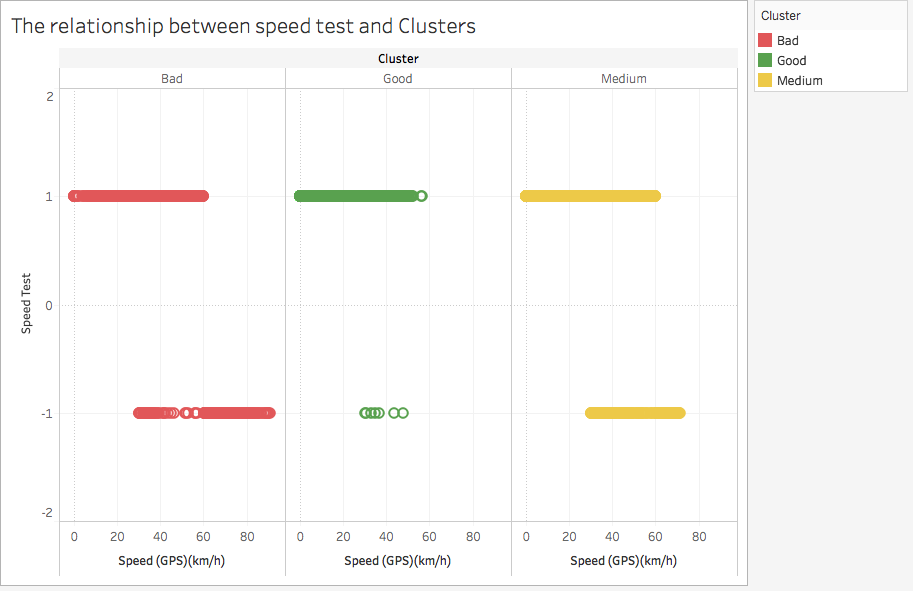
\includegraphics[height=.5\textwidth]{image/clusterresult}
\caption{The relationship between the speed test and the three clusters.}
\label{fig:cluster_result}
\end{figure}


\subsection{Work Flow Design}
The completed work flow is displayed in the Figure \ref{fig:workflow}. The CSV Reader is the module that allows CSV file to be inserted into the work flow and perform the data preprocessing at the same time. The Concatenate module will combine the drivers vehicle telemetry data. The K Means Algorithm module will perform clustering to categorized the data into three groups. The number of groups is set in the module configuration. Figure \ref{fig:kmean} shows the configuration of the K Means Algorithm module.

\begin{figure}[hbt!]\centering
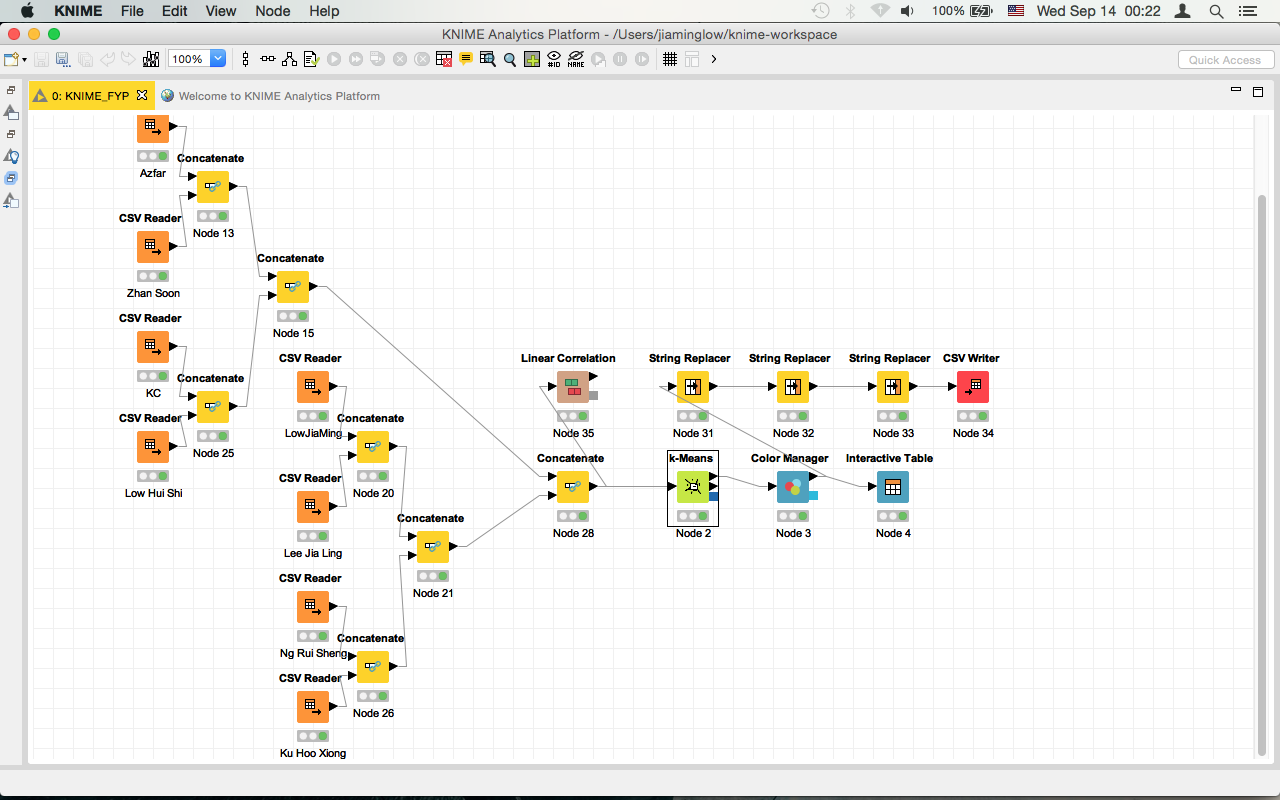
\includegraphics[width=.75\textwidth]{image/KNIMEfile}
\caption{The completed workflow for classify the driving operation model.}
\label{fig:workflow}
\end{figure}

\begin{figure}[hbt!]\centering
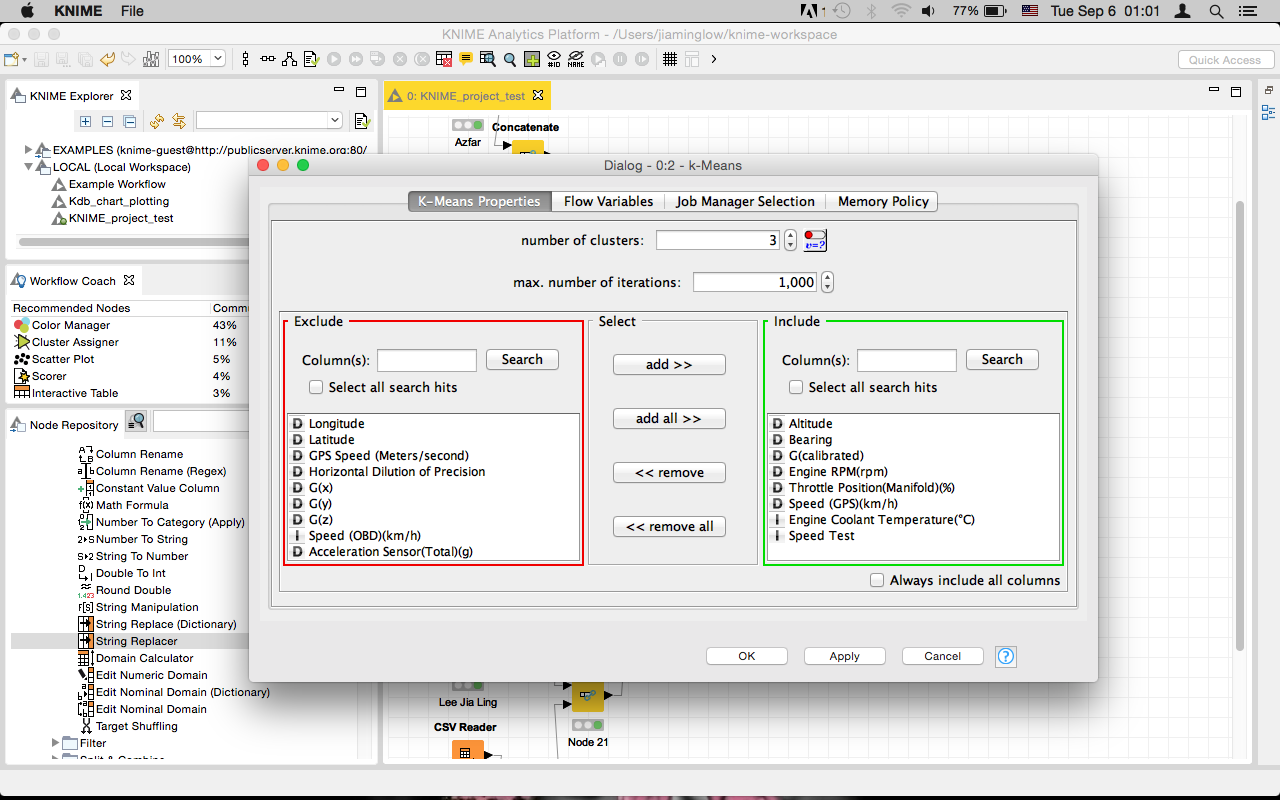
\includegraphics[width=.75\textwidth]{image/KNIMEkmean}
\caption{K Means Algorithm module setting.}
\label{fig:kmean}
\end{figure}



\section{Driver Driving Behaviour Profiling}
In this project, the driver driving behaviour profile can be determined by some condition. %The total of good vehicle condition data (VCD) should over at least 55\% of the total records of the particular driver collected, then the driver will be categorized as low risk driver. It also means that 
If the total of good VCD is greater than the total of medium VCD and bad VCD at least 10\% of the total records, the particular driver will be categorized as low risk driver. If the amount of good VCD do not fulfil the condition, the total of medium VCD and bad VCD will be chosen for classifying the driver. The total of medium vehicle VCD should over at least 55\% of the total medium VCD and bad VCD, then the driver will be categorized as medium risk driver. Otherwise, the driver will be categorized as high risk driver.

After trying few method to determine the driver driving behaviour profile, this method is the most suitable among the method. It is because there are two comparison to be performed to get the driver driving behaviour profile. The first comparison will determine whether the driver is low risk driver. In order to fulfil the condition of the first comparison, the good VCD should over 55\% of the total records. If not, the rest of the records will be used for determining whether the driver is medium risk or high risk driver. The medium VCD is required to have 55\% among the medium VCD and bad VCD, then the driver only can be categorized as medium risk driver.

The table \ref{tbl:result} shows the result of the total number of driving records for each cluster and the driver driving profile.

\begin{table}[h!]
\begin{tabular}{|l|c|c|c|c|}
\hline
Driver & Good Model & Medium Model & Bad Model & Driver Driving Profile \\

\hline
Candidate 1 & 239 & 138 & 249 & High Risk\\

\hline
Candidate 2 & 178 & 120 & 271 & High Risk\\
  
\hline
Candidate 3 & 178 & 156 & 237 & High Risk\\

\hline
Candidate 4 & 372 & 207 & 67 & Low Risk\\

\hline
Candidate 5 & 553 & 294 & 95 & Low Risk\\

\hline
Candidate 6 & 144 & 446 & 88 & Medium Risk\\

\hline
Candidate 7 & 372 & 304 & 205 & Medium Risk\\

\hline
Candidate 8 & 163 & 445 & 103 & Medium Risk\\

\hline
\end{tabular}
\label{tbl:result}
\caption{The result of the driver driving behaviour profiling.}    
\end{table}

One of the ways to determine the driver driving behaviour profile has been tried. The method is using the average of the records among the three clusters to compare with the total amount of each cluster . If the good VCD exceeds the average point, the particular driver will be classified as low risk driver. It is same to every clusters.

This method is not suitable for determining the driver driving behaviour profile as there will have same cases difficult to classified the drivers' risk level. In Figure \ref{fig:Tresult}, Candidate 1 will be hard to classify the driver's risk level as the good VCD and bad VCD exceed the average at the same time. So, this method is not suitable.
 
\begin{figure}[hbt!]\centering
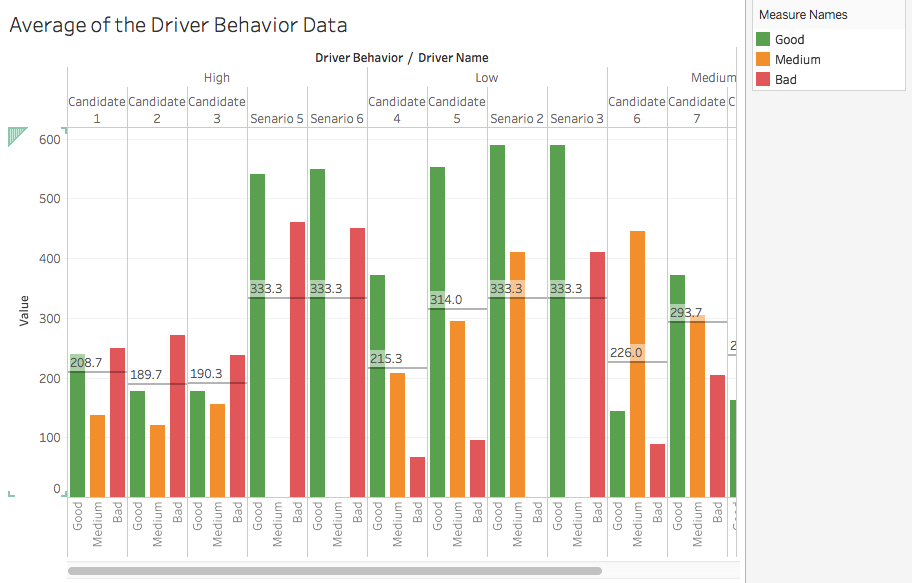
\includegraphics[width=.75\textwidth]{image/Tresult}
\caption{The result of the driver driving behaviour profiling by using Tableau side-by-side bar with average point.}
\label{fig:Tresult}
\end{figure} 